\documentclass{article}
\usepackage[utf8]{inputenc}
\usepackage{amsmath}
\usepackage{mathtools}
\usepackage{bm}
\usepackage{hyperref}
\author{Sujatha}
\title{Skewness and Kurthosis}
\begin{document}
\maketitle
\section{Skewness}
Skewness is the standardised third moment. It is a measure of asymmetry of the probability distribution. A positive skewness means there is more It is defined as follows
\begin{align*}
 \gamma_1 = E\left[\left(\dfrac{X -\mu}{\sigma}\right)^3  \right]
\end{align*}
\begin{figure}
\begin{center}
 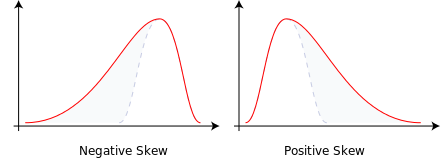
\includegraphics{skewness.png}
 % Negative_and_positive_skew_diagrams_(English).svg: 0x0 pixel, 300dpi, 0.00x0.00 cm, bb=
 \caption{source:wiki}
\end{center}
\end{figure}
\section{Kurtosis}
Kurtosis is the standardised fourth moment. It is a measure that describes the shape of the distributions tail in relation to its overall 
shape. It is defined as follows
\begin{align*}
 \gamma_1 = E\left[\left(\dfrac{X -\mu}{\sigma}\right)^4  \right]
\end{align*}
\end{document}